\documentclass[]{AVSSimReportMemo}
\usepackage{AVS}

\newcommand{\ModuleName}{orbitAxisSpin}
\newcommand{\subject}{Guidance Module to Perform a Constant Spinning about an Orbit Axis}
\newcommand{\status}{Initial Version}
\newcommand{\preparer}{M. Cols}
\newcommand{\summary}{Generate the attitude reference to achieve a spinning motion about a primary orbit frame axis. A chosen reference axis $\hat{b}_{j} = \hat{b}_{spin}$ is to line up with the orbit axis $\hat{o}_{i} = \hat{o}_{spin}$, and rotate a desired rate $\omega_{spin}$}


\begin{document}

\makeCover


%
%	enter the revision documentation here
%	to add more lines, copy the table entry and the \hline, and paste after the current entry.
%
\pagestyle{empty}
{\renewcommand{\arraystretch}{2}
\noindent
\begin{longtable}{|p{0.5in}|p{4.5in}|p{1.14in}|}
\hline
{\bfseries Rev}: & {\bfseries Change Description} & {\bfseries By} \\
\hline
Draft & initial copy & M. Cols \\
\hline

\end{longtable}
}

\newpage
\setcounter{page}{1}
\pagestyle{fancy}

\tableofcontents
~\\ \hrule ~\\

\begin{figure}[htb]
	\centerline{
	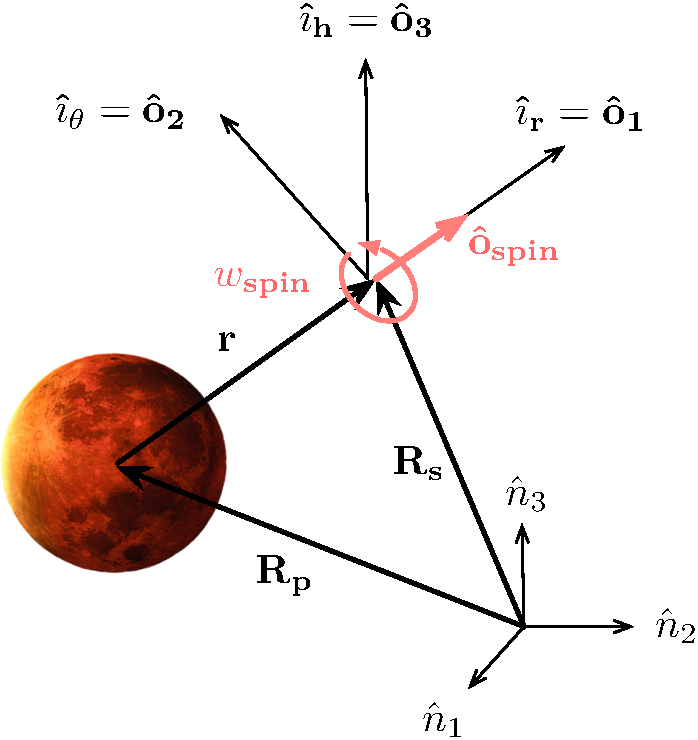
\includegraphics[width=5cm]{Figures/Fig1}
	}
	\caption{Illustration of spinning about the nadir orbit axis $\bm\hat{\imath}_{r}$ of the Hill orbit frame $\mathcal{H}$  at a constant rate $\omega_{\textrm{spin}}$.}
	\label{fig:Fig1}
\end{figure}

\section{Introduction}
In this note a method is discussed on how to compute the reference frame angular rate $\bm\omega_{R/N}$ and acceleration $\dot{\bm\omega}_{R/N}$ to achieve a particular family of stabilized spin motion. This module receives as input a constant pointing orbit-frame $\mathcal{R}_{0}$. The goal is now to create a new reference $\mathcal{R}$ that spins about any of the orbit axes that conform $\mathcal{R}_{0}$  at a constant rate $\omega_{\textrm{spin}}$. Let us call the spinning orbit axis $\hat {o}_{\textrm{spin}}$. Note that the presented method is general enough to use any of the Hill $\mathcal{H}:\{ \hat{\bm\imath}_{r}, \hat{\bm\imath}_{\theta}, \hat{\bm\imath}_{h} \}$ or Velocity $\mathcal{V}:\{ \hat{\bm\imath}_{n}, \hat{\bm\imath}_{v}, \hat{\bm\imath}_{h} \}$ orbit frame orientations as the input reference. Figure 1 illustrates the case in which $\mathcal{R}_{0} = \mathcal{H}$ and the spinning is about the nadir axis $\hat {o}_{\textrm{spin}} = \hat{\bm\imath}_{r}$.

\section{Reference Frame Generation}
\subsection{Angular Velocity and Acceleration Descriptions}
The reference frame $\mathcal{R}$ is defined above, and the attitude reference frame tracking control requires the angular rate $\bm\omega_{R/N}$ and acceleration $\dot{\bm\omega}_{R/N}$. 
Let the MRP attitude set, angular velocity vector and angular acceleration vector associated with the constant pointing reference be $\bm\sigma_{
R_{0}/N}$, $\bm\omega_{R_{0}/N}$ and $\bm\dot{\omega}_{R_{0}/N}$ respectively.
The angular velocity of the spinning reference frame is thus given by:
\begin{subequations}
	\label{eq:omegaRN}
	\begin{equation}
		\bm\omega_{R/N} = \bm\omega_{\textrm{spin}} + \bm\omega_{R_{0}/N} 
	\end{equation}
	\begin{equation}
		\bm\omega_{R/N} = {\omega}_{\textrm{spin}}\hat{o}_{\textrm{spin}} + \bm\omega_{R_{0}/N}
	\end{equation}
\end{subequations}
Since $\hat {o}_{\textrm{spin}}$ is aligned with one of the orbit axis defining $\mathcal{R}_{0}$, taking the inertial derivative of ~\eqref{eq:omegaRN}:
\begin{subequations}
	\label{eq:domegaRN}
	\begin{equation}
		\dot{\bm\omega}_{R/N} = \dot{\bm\omega}_{\textrm{spin}} +\dot{\bm\omega}_{R_{0}/N} 
	\end{equation}
	\begin{equation}
		\dot{\bm\omega}_{R/N} = \frac{^{\mathcal{R}_{0}} \textrm{d}}{\textrm{dt}} (\omega_{\textrm{spin}}\bm\hat{o}_{\textrm{spin}}) + \bm\omega_{R_{0}/N}\times (\omega_{\textrm{spin}}\bm\hat{o}_{\textrm{spin}}) + \bm{\dot\omega}_{R_{0}/N}
	\end{equation}
\end{subequations}

\subsection{MRP Attitude Set}
Let $\phi_{\textrm{spin}}$ be the current spin angle that the reference frame has rotated about its spin axis $\hat o_{\textrm{spin}}$. The final reference frame orientation is eventually given by
\begin{equation}
	\label{eq:dbeta}
	[RN] =  [M_{\hat{o}_{\textrm{spin}}} (\phi_{\textrm{spin}})][R_{0}N]
\end{equation}
where $[R_{0}N]$ is the Direction Cosine Matrix associated with the orbit axis pointing attitude set, and $M_{\hat{o}_{\textrm{spin}}}$ is the principal axis rotation matrix about $\hat o_{\textrm{spin}}$. Assuming a constant spin rate, the spin angle is propagated using the simple Euler integration scheme
\begin{equation}
	\label{eq:dbeta}
	\phi_{\textrm{spin, n+1}} = \phi_{\textrm{spin, n}} + \omega_{\textrm{spin}}\Delta t
\end{equation}
With $[RN]$ defined, the MRP attitude set $\sigma_{R/N}$ can readily be computed.

\section{Spin Angle Initialization}



The question remains on how to initialize the spin angle $\phi_{\textrm{spin}}$. Since the initialization of the spin angle requires of knowing the actual body frame and doing it in a completely general way is not feasible, a separate algorithm is used.
Being $\mathcal{B}$ the body frame and $\mathcal{R}_{0}$ the orbit frame orientations, let us set $\hat{b}_{\textrm{spin}}$ as the principal body axis that is to be aligned with the principal orbit axis $\hat{o}_{\textrm{spin}}$. The triodes of axes $\hat b_{i}$ and $\hat o_{i}$ are labeled so that the first index determines the spin axis, i.e. $\hat b_{1} =\hat b_{\textrm{spin}}$ and $\hat o_{1} =\hat o_{\textrm{spin}}$. The remaining two indices are set to yield a right-handed coordinate frame.\par

Let $\mathcal{R}$ be the reference orientation in which $\hat o_{1}$ orbit axis and $\hat b_{1}$ body axis are lined up. Using the definition where $RN(i)$ is the $i_{th}$ row of the $[RN]$ DCM matrix:
\begin{equation}
	\label{eq:dbeta}
	RN(\hat b_{1}) = R_{0}N(\hat o_{1}) 
\end{equation}
\begin{equation}
	\label{eq:dbeta}
	RN(\hat b_{2}) = R_{0}N(\hat o_{2}) 
\end{equation}
\begin{equation}
	\label{eq:dbeta}
	RN(\hat b_{3}) = RN(\hat b_{1}) \times RN(\hat b_{2})
\end{equation}

Now, the desired orientation for the body-frame $[RN]$ and the current one $[BN]$ are completely determined.\newline
\begin{figure}[htb]
	\centerline{
		\includegraphics[width=10cm]{Figures/FigRB}
	}
	\caption{Current body-frame $[BN]$ and goal reference frame $[RN]$}
	\label{fig:Fig2}
\end{figure} 
\newline
Let us designate the initial angle between $\hat {b}_{\textrm{spin}}$ and $\hat {o}_{\textrm{spin}}$, before tha alignment, as $\phi_{align}$. Once a principal rotation of $\phi_{align}$ is applied to the body-frame for the purposes of this module, i.e. $\hat {b}_{\textrm{spin}}$ becomes coincident with $\hat {o}_{\textrm{spin}}$ , the other two body axes are only assured to be contained in the plane normal to the spinning axis. Let us eventually define $\phi_{\textrm{spin}}$ as the smallest angle to align the remaining axes with their corresponding desired ones.
At this point, it is important to recall that any general alignment between reference frames can be achieved through a single rotation about a principal rotation axis and that this rotation can be either of $\phi$ or $( 2\pi - \phi)$, which correspond to the short and long way respectively. \newline
The purpose of the algorithm presented in this section is to ensure that the spinning is always initialized to go the short way.
Let us first compute the alignment angle between the prospective spinning axes:
\begin{equation}
	\label{eq:phi_align}
	\phi_{align} = \arccos{(RN(\hat b_{1}) \cdot BN(\hat b_{1}))}
\end{equation}
Note that $RN(\hat b_{1})$ and $RN(\hat b_{1})$ are vectors already normalized.
And the principal rotation vector for the alignment is:
\begin{equation}
	\label{eq:e_hat_align}
	\hat{e}_{align} = RN(\hat b_{1}) \times BN(\hat b_{1})
\end{equation}
\begin{equation}
	\label{eq:e_align}
	\bm{e}_{align} = \phi_{align}\hat{e}_{align} 
\end{equation}
Let us designate $\mathcal{F}$ as the intermediate frame where $\hat {b}_{\textrm{spin}}$ and $\hat {o}_{\textrm{spin}}$ are aligned. 
\newline
\begin{figure}[htb]
	\centerline{
		\includegraphics[]{Figures/FigFB}
	}
	\caption{Current body-frame $\mathcal{B}$  and intermediate frame $\mathcal{F}$ }
	\label{fig:Fig3}
\end{figure} 
\newline
Through the following function from the Rigid Body Kinematic library in Reference~\citenum{schaub}, the DCM corresponding to the previous principal rotation vector is computed:
\begin{equation}
	\label{eq:BF}
	[BF] = \textrm{PRV2C}(\bm{e}_{align})
\end{equation}
Now, we can align the spinning axes:
\begin{equation}
	\label{eq:FN}
	[FN] = [BF]^{T}[BN]
\end{equation}
Next, let us compute the relative orientation between the intermadiate frame $\mathcal{F}$ and the reference $\mathcal{R}$
\begin{equation}
	\label{eq:RF}
	[RF] = [RN][FN]^T
\end{equation}

Making use again of the same Rigid Body Kinematic Library, we compute the associated principal rotation vector (direction ang angle):
\begin{equation}
	\label{eq:e_spin}
	\bm{e}_{spin} = \textrm{C2PRV}([RF])
\end{equation}
Where $ \phi_{spin, 0} = |\bm{e}_{spin}| $ shall be checked if corresponds to the short or long rotation:
if the angle between $\bm{e}_{spin}$ and $[RN(\hat{b}_{spin})]$ is 180 deg, then the computed $\phi_{spin}$ corresponds to the latter case and its sign needs to be switched in order to guarantee following the shortest path. \newline
Mathematically, the check is accomplished through a simple if-statement:

If
$$\bm{e}_{spin} \cdot RN[\hat{b}_{spin}] < 0 $$

Then,
$$\phi_{spin,0} = -\phi_{spin, 0}$$

Where, recall that $RN[\hat{b}_{spin}]$ is a base vector and the first expression is thus a dot product between vectors, directly related to the cosinus of the angle between them.

\begin{figure}[htb]
	\centerline{
		\includegraphics[width=5cm]{Figures/FigRF}
	}
	\caption{Goal reference-frame $\mathcal{R}$  and intermediate frame $\mathcal{F}$ }
	\label{fig:Fig4}
\end{figure} 


\bibliographystyle{unsrt}
\bibliography{references}

\end{document}
